\question (浙江大学,2000年)存储器的存取时间是指
\par\twoch{存储器的读出时间}{存储器的写入时间}{存储器进行连续读或连续写操作所允许的最短时间间隔}{\textcolor{red}{存储器进行一次读或写操作所需的平均时间}}
\begin{solution}D。
存取时间是指存储器进行一次读或写操作所需的平均时间。C选项是存取周期的定义。
\end{solution}
\question 某32位微型机地址码为32位,若使用32K×8位的RAM芯片进行字扩展成存储器,则该机所允许的最大主存容量是
\par\twoch{32KB}{16MB}{512MB}{\textcolor{red}{4GB}}
\begin{solution}D。 想要知道最大主存容量就只需要知道存储单元大小和存储单元个数就能得出。
由于存储器是由32K×8位的RAM芯片进行字扩展而成的,那么存储单元大小就为8位,即1B。
又地址码为32位,得出存储单元个数为2\^{}32,所以最大出存容量为2\^{}32×1B=4GB。
\end{solution}
\question 某1K×8位(1K×8矩阵)的半导体存储芯片内部译码驱动方式采用``线选法'',需要(
)根选择线才能选择存储芯片内的任一存储单元
\par\twoch{10}{32}{64}{\textcolor{red}{1024}}
\begin{solution}D。
这里要注意,问的是选择线不是地址线。线选法,即用一根字选择线来选中一个存储单元的所有存储元,题中1K×8位的存储芯片共有1K个存储单元,故需1K=1024根选择线才能够选择该存储芯片内的任一存储单元。
如果题目问的是地址线的话,无论``线选法''还是``重合法''答案都是一样的,通过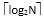
\includegraphics[width=0.45833in,height=0.18750in]{computerassets/018a53d6590bef422ef084b772e297be.jpeg}可以算出地址线所需要的根数。
\end{solution}
\question 假定用若干16K×8位的存储器芯片组成一个64K×8位的存储器,芯片各单元交叉编址,则地址BFFF所在的芯片的最小地址为
\par\twoch{0000H}{0001H}{0002H}{\textcolor{red}{0003H}}
\begin{solution}D。 首先计算下需要用多少块16K×8位的存储器才能组成64K×8位的存储器:
(64×8)/(16×8)=4,又芯片各单元交叉编址。也就是 0000 0000 0000
0000B在第一块 0000 0000 0000 0001B在第二块 0000 0000 0000 0010B在第三块
0000 0000 0000 0011B在第四块 0000 0000 0000 0100B在第一块 0000 0000 0000
0101B在第二块 0000 0000 0000 0110B在第三块 0000 0000 0000
0111B在第四块。 \ldots{}\ldots{} 可以看出,最后两位其实是片选位。
我们将BFFF转换为16进制地址为:1011 1111 1111
1111B,该地址应该是在第四块芯片上,它的最小地址为0000 0000 0000
0011B,即0003H。故本题选D。
\end{solution}
\question 某计算机主存地址16位,每个存储单元有8位,即按字节编址。如果用1K×4位的RAM芯片构成该计算机的最大主存空间,片选逻辑的输入需要(
)位地址
\par\twoch{4}{\textcolor{red}{6}}{8}{16}
\begin{solution}B。
因为主存地址为16位,所以主存地址空间大小为64K个存储单元,每个存储单元占8位。因此需要的芯片数为(64K/1K)×(8/4)=128。存储器在字方向上扩展了64倍,因而片选逻辑需要log2(64)=6位地址。
\end{solution}
\question 在1K×8位的存储器芯片中,采用双译码方式,译码器的输出信号总数有( )条
\par\twoch{1024}{\textcolor{red}{64}}{32}{10}
\begin{solution}B。
采用双译码地址,可以减少地址选择线的数目。在双译码结构中,设译码器的总的输入信号有n条,地址译码器分成两个,则每个译码器有n/2个输入,就可以有2\^{}(n/2)个输出状态,则两个地址译码器就有2\^{}(n/2)×2\^{}(n/2)个输出状态,对应存储单元数。
1K =
2\^{}(n/2)×2\^{}(n/2)=32×32,要注意本题问的不是n是多少,题目问的是译码器的输出信号(即2\^{}(n/2)的值),即32+32=64。
\end{solution}
\question 需要一个16M×8位的存储器,现有存储芯片为1M×8位。那么主存储器的地址中用于选择存储芯片的位数为
\par\twoch{\textcolor{red}{4}}{16}{20}{24}
\begin{solution}A。 解法一:
用1M×8位的存储芯片组成16M×8位的存储器,需要进行字扩展,需要的存储芯片的个数=(16M×8位)/(1M×8位)=16。那么用于选择存储芯片的位数为log2
(16)=4。故本题选A。 解法二:
存储器芯片容量为1M×8=2\^{}20×8,需要20根地址线,地址长度需要20位。
主存储器的容量为16M×8=2\^{}24×8,需要24根地址线,地址长度需要24位。其中20为位存储器芯片地址,剩余4位即为片选地址。故本题选A。
\end{solution}
\question 下列哪些信号与片选信号的形成有关
\par\twoch{CPU访存控制信号}{CPU访存地址信号}{\textcolor{red}{A和B}}{以上都不对}
\begin{solution}C。
片选信号的形成与A和B都有关系。只有当CPU需要访存时,才需要选择存储芯片,而访存时选择哪个存储芯片需要根据CPU访存时给出的地址信号来决定。
\end{solution}
\question 某1K×1位(32×32矩阵)的存储芯片内部移码驱动方式采用``重合法''时,需要(
)根选择线才能选择存储芯片内的任一存储单元
\par\twoch{10}{32}{\textcolor{red}{64}}{1024}
\begin{solution}C。
重合法通过行地址和列地址来共同选中一个存储单元,题中1K×1位存储芯片内部为32×32矩阵,故行、列选择线均为32根,故需要32+32=64根选择线才能选中该芯片内的任一存储单元。
\end{solution}
\question 设CPU有16根地址线、8根数据线。主存地址空间分配:6000H~67FFH为系统程序区;6800H~6BFFH为用户程序区。从下列存储芯片中,分别合理选用下述存储芯片
Ⅰ.1K×4位RAM Ⅱ.2K×8位RAM Ⅲ.8K×8位RAM Ⅳ.2K×8位ROM Ⅴ.1K×8位ROM
Ⅵ.8K×8位ROM
\par\fourch{Ⅰ×2用作系统程序区,Ⅳ×1用作用户程序区}{\textcolor{red}{Ⅳ×1用作系统程序区,Ⅰ×2用作用户程序区}}{Ⅳ×1用作系统程序区,Ⅴ×1用作用户程序区}{Ⅱ×1用作系统程序区,Ⅴ×1用作用户程序区}
\begin{solution}解法一: 如下图所示:
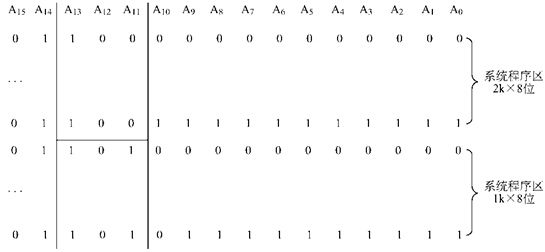
\includegraphics[width=5.67708in,height=2.62500in]{computerassets/bd12baddaa6720a3d704b4d11c38d257.jpeg}
6000H~67FFH为系统程序区的范围,故应选1片2K×8位的ROM芯片。
6800H~6BFFH为用户程序区的范围,故应选2片1K×4位的RAM芯片。
需要注意的是,存放系统程序或各类常数使用ROM芯片,存放用户程序应该选用RAM芯片。
解法二: 6000H~67FFH为系统程序区的范围,67FFH-6000H+1H=800H=8×16\^{}2。
6800H~6BFFH为用户程序区的范围,6BFFH-6800H+1H=400H=4×16\^{}2。
又数据线为8根,即系统程序区需用2K×8位,用户程序区需用1K×8位。
所以系统程序区,应选1片2K×8位的ROM芯片;用户程序区,应选2片1K×4位的RAM芯片。
\end{solution}
\question 下图是某存储芯片的引脚图,这个存储芯片的类型是(
~),且下图中的``?''为( ~)。注:NC表示未用

~
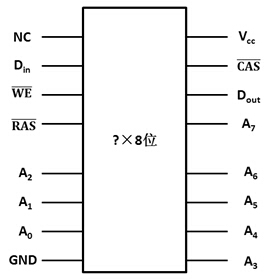
\includegraphics[width=2.80208in,height=2.91667in]{computerassets/169329cf2d8e984977db0414ac033cd3.jpeg}
\par\fourch{ROM,128}{ROM,256}{RAM,128}{\textcolor{red}{RAM,256}}
\begin{solution}D。
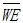
\includegraphics[width=0.23958in,height=0.23958in]{computerassets/b350bfb1f8737a0025f7d2cebbbeacc0.jpeg}为写允许信号,这个是ROM所没有的引脚。故该存储芯片为RAM。
因为这里有8根地址线,所以此存储芯片的存储单元为2\^{}8=256,故上图中的``?''为256。
\end{solution}
\question 设CPU地址总线有24根,数据总线有32根,用512K×8位的RAM芯片构成该机的主存储器,则该机主存最多需要(
)块存储芯片
\par\twoch{64}{\textcolor{red}{128}}{256}{512}
\begin{solution}B。 本题的本质还是a×b位的存储器由多少块c×d位的存储芯片组成。
CPU地址总线有24根,那么地址空间为2\^{}24,数据总线有32根,那存储单元为32位,也就是说该机主存最大容量为2\^{}24×32位。
那么所需要的存储芯片数=2\^{}24×32位/(512K×8位)=
2\^{}24×32/(2\^{}19×8)=128,故本题选B。
\end{solution}
\question 一个存储器系统中,常常同时包含ROM和RAM两种类型的存储器,如果用1K×8位的ROM芯片和1K×4位的RAM芯片,组成4K×8位的ROM和1K×8位RAM的存储系统,按先ROM后RAM进行编址。采用3:8译码器选片,译码信号输出信号为Y0\textasciitilde{}Y7,其中Y4选择的是
\par\twoch{第一片ROM}{第五片ROM}{第一片RAM}{\textcolor{red}{第一片RAM和第二片RAM}}
\begin{solution}D。 所需ROM的芯片数=(4K×8位)/(1K×8位)=4片,字扩展。
所需RAM的芯片数=(1K×8位)/(1K×4位)=2片,位扩展。
采用3:8译码器,又已知``按先ROM后RAM进行编址'',则Y0选中第一片ROM,\ldots{}\ldots{},Y3选中第四片ROM。两片RAM(1K×4位)作为一个存储体,Y4选中该存储体。
\end{solution}
\question 某32位微型机地址码为22位,使用256K×16位的SRAM芯片组成其存储系统,下列译码器中最合适的是
\par\twoch{3:8译码器}{\textcolor{red}{4:16译码器}}{5:32译码器}{6:64译码器}
\begin{solution}B。
``32位微型机地址码为22位'',得出该微型机的存储系统容量为2\^{}22×32位。
使用256K×32位的SRAM芯片组成2\^{}22×32位的存储系统,需要(2\^{}22×32位)/(256K×16位)=32片。其中每两片位并联的方式构成256K×32位的存储体,然后用16组这样的存储体构成2\^{}22×32位的存储体。然后通过译码器产生片选信号来用于存储体的选择,故最合适的是有16种输出信号的译码器,即4:16译码器,因此本题选B。
\end{solution}
\question (华中科技大学,2002年)4片16K×8的存储芯片,可以设计成( )容量的存储器
\par\twoch{\textcolor{red}{32K×16}}{16K×16}{32K×8}{16K×8}
\begin{solution}A。
首先,可以2片一组进行位扩展,扩展之后为2片16K×16位的芯片;然后这2个芯片再进行字扩展为32K×16位,故选项A正确,其余选项均不合要求。
\end{solution}
\question (北京理工大学)在1K×8的存储芯片中,采用双译码方式,译码器的输出信号有(
)条
\par\twoch{1024}{\textcolor{red}{64}}{32}{10}
\begin{solution}B。
双译码就是重合法,其通过行线和列线共同选中存储器任一单元。1K=2\^{}5×2\^{}5=32×32,也就是构造出32×32的矩阵,行线32根,列线32根,共64根。
\end{solution}
\question (西安电子科技大学,2005年)80386DX是32位系统,当在该系统中用8KB的存储芯片构造32KB的存储体时,应完成存储器的(
)设计
\par\twoch{\textcolor{red}{位扩展}}{字扩展}{字位扩展}{字位均不扩展}
\begin{solution}A。
本题的意思就是将8K×8位的芯片扩展成8K×32位的芯片,所以应完成存储器的位扩展。
\end{solution}
\question (南京航空航天大学,1999年)地址总线为A15(高位)~A0(低位),若用1K×4位的存储芯片组成4KB的存储器,地址总线的高位做片选,则加在各存储芯片上的地址线是
\par\twoch{A15~A0}{A11~A0}{\textcolor{red}{A9~A0}}{A8~A0}
\begin{solution}C。
对于X×Y的芯片,X的大小与地址线相关,Y的大小与数据线相关。对于此题,因为2\^{}10B=1KB,故选取地址线的低10位A9~A0作为各存储芯片上的地址线,高位作为片选线。
\end{solution}
\question 存储器采用部分译码法片选时,( )
\par\twoch{不需要地址译码器}{不能充分利用存储器空间}{\textcolor{red}{会产生地址重叠}}{CPU的地址线全参与译码}
\begin{solution}C。
部分译码即只用高位地址的一部分参与译码,而另一部分高位地址与译码电路无关,因此出现一个存储单元对应多个地址的现象,这种现象被称为地址重叠(如00111和01111,前两位不参与译码,导致一个存储单元对应多个地址)。
\end{solution}
\question 已知单个存储体的存取周期为T,CPU连续从四体高位交叉存储器中取出N个字需要时间为
\par\twoch{4T}{(N-1)T}{\textcolor{red}{NT}}{}
\begin{solution}C。
高位交叉编址的多体存储器(其实这里说交叉不是很准确,说顺序存储更好理解),当存储器只与CPU交换信息时,其带宽与单体存储器相等。只有当合理调度,使得CPU与外部设备同时访问存储器的不同体时,才能发挥其优势,如在某一时刻CPU在和第0个体交换数据,而此时第1个体正在和I/O交换数据,从而实现个体的并行工作。
若采用低位交叉编址的存储器,连续读取n个字所需要的时间t1为 t1=T+(n-1)t
若采用高位交叉编址的存储器,连续读取n个字所需要的时间t2为 t2=nT
T为存取周期,t为总线传送周期。
详细请参考《计算机组成原理高分笔记》3.5节。
\end{solution}
\question CPU和主存的连接如下图所示,左起第二块SRAM的地址空间为:
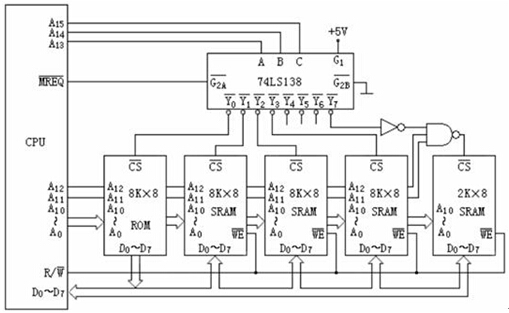
\includegraphics[width=3.33333in,height=2.05208in]{computerassets/abb8d51d2db36dda74a8b1a0ac81edd9.jpeg}
\par\fourch{2000~3FFF}{3000~3FFF}{4000~4FFF}{\textcolor{red}{4000~5FFF}}
\begin{solution}D。
若要选中第二块SRAM,需要被Y2信号选中,即A13\textasciitilde{}A15需要为010,即地址空间为0100
0000 0000 0000 \textasciitilde{}0101 1111 1111
1111,即4000\textasciitilde{}5FFF。故本题选D。
\end{solution}
\question 某主存储器容量为256K×8位,由32K×8位芯片组成,设其中一芯片在片选地址为110时获得片选信号。该芯片占用的地址空间为
\par\twoch{30000~3FFFF}{80000~8FFFF}{\textcolor{red}{30000~37FFF}}{80000~87FFF}
\begin{solution}C。
由题意可知,该主存储器有256K个单元,则需要地址位数为log2(256K)=18位。片选地址为110,剩余15位为片内地址。很容易知道首地址为11
0000 0000 0000 0000,末地址为11 0111 1111 1111
1111。换成16进制为30000和37FFF。本题选C。
\end{solution}
\question 下列的说法中,正确的是 Ⅰ.双端口存储器可以同时异步访问同一存储单元
Ⅱ.双端口存储器当两个端口的地址码相同时,必然会发生冲突
Ⅲ.高位多体交叉存储器的设计依据了程序的局部性原理
Ⅳ.高位四体交叉存储器可能在一个存储周期内连续访问4个模块
\par\twoch{Ⅰ和Ⅲ}{Ⅱ和Ⅲ}{\textcolor{red}{Ⅰ和Ⅳ}}{只有Ⅰ}
\begin{solution}C。 高位多体交叉存储器仍然是顺序存储器。
双口RAM最大的特点是存储数据共享。一个存储器配备两套独立的地址、数据和控制线,允许两个独立的CPU或控制器同时异步地访问存储单元,故I正确。当两个端口同时对相同的单元进行读操作时,则不会发生冲突,Ⅱ错误。高位多体交叉存储器由于是在单个存储器中字是连续存放的,所以不能保证程序的局部性原理;而低位多体交叉存储器由于是交叉存放的,所以能很好地满足程序的局部性原理,Ⅲ错误。高位四体交叉存储器虽然不能满足程序的连续读取,但仍可能一次连续读出彼此地址相差一个存储体容量的4个字,只是这么读的概率较小,Ⅳ正确。
\end{solution}
\question 假定用若干个16K×8位的存储器芯片组成一个64K×32位的存储器,芯片内各单元连续编址,则地址BFF0H所在芯片中的最小地址为
\par\twoch{4000H}{6000H}{\textcolor{red}{8000H}}{A000H}
\begin{solution}C。 首先计算下需要用多少块16K×8位的存储器才能组成64K×8位的存储器:
(64×32)/(16×8)=16。
每4片一组分成4组,每组按位扩展方式组成一个16K×32位的模块,4个模块按字扩展方式构成64K×32位的存储器。问题问的是BFF0H所在芯片的最小地址,BFF0H地址指向的其实是模块,而不是某个16×8位的芯片,故只需要求出该模块的最小地址即可。又芯片内各单元连续编址,则地址中的模块位为前两位(因为有4个模块),把BFF0H写成16进制地址为:1011
1111 1111 0000B,其对应模块为10,该模块的最小地址为 1000 0000 0000
0000B,十六进制地址为8000H,故本题选C。
\end{solution}
\question 某计算机存储器按字节编址,主存地址空间大小为64MB,现用4M*8位的RAM芯片组成32MB的主存储器,则存储器地址寄存器MAR的位数至少是(
)
\par\twoch{22位}{23位}{25位}{\textcolor{red}{26位}}
\begin{solution}本题有个``陷阱'',相信不少考生会以32MB的实际主存来计算,从而得到答案为25位,这种解法是错误的。尽管多余的32MB没有使用,但是也得防备以后要用。知道以64MB来计算就很好做了。由于采用字节寻址,所以寻址范围是64MB,而226B=64MB,故存储器地址寄存器(MAR)的位数至少是26位。
\end{solution}
\question 假定用若干个2K×4位芯片组成一个8K×8位的存储器,则地址0B1FH所在芯片的最小地址是(
)
\par\twoch{0000H}{0600H}{0700H}{\textcolor{red}{0800H}}
\begin{solution}由2K×4位芯片组成8K×8位芯片,需要8片2K×4位芯片,即分为4组,每组由两片2K×4位芯片组成2K×8位芯片。其中每组中两片2K×4位芯片由同一地址访问。
4组的地址格式:0000 0000 0000 0000 0000 0111 1111 1111(第一组) 0000
1000 0000 0000 0000 1111 1111 1111(第二组) 0001 0000 0000 0000 0001
0111 1111 1111(第三组) 0001 1000 0000 0000 0001 1111 1111
1111(第四组) 0B1FH的地址格式是0000 1011 0001
1111,可知它属于第二组中的一个地址,这个地址所在芯片的最小地址为0000
1000 0000 0000,即0800H。
\end{solution}
\question 假定主存地址为32 位,按字节编址,主存和Cache
之间采用直接映射方式,主存块大小为4 个字,每字32 位,采用回写(Write
Back)方式,则能存放4K 字数据的Cache 的总容量的位数至少是()
\par\twoch{146k}{\textcolor{red}{147K}}{148K}{158K}
\begin{solution}Cache 和主存的映射方式。直接映射方式地址映象规则:
主存储器中一块只能映象到Cache 的一个特定的块中。(1)
主存与缓存分成相同大小的数据块。(2)
主存容量应是缓存容量的整数倍,将主存空间按缓存的容量分成区,主存中每一区的块数与缓存的总块数相等。(3)
主存中某区的一块存入缓存时只能存入缓存中块号相同的位置。
\end{solution}
